\documentclass[a4paper,11pt]{report}
\usepackage[slovene]{babel}
\usepackage{listings}
\usepackage{graphicx}
\usepackage[section]{placeins}
\usepackage{footnote}
\makesavenoteenv{tabular}

\newcommand{\ttitle}{Vzorec bla dela}
\newcommand{\tauthor}{Matjaž Kralj}
\newcommand{\autfont}{\Large}
\newcommand{\titfont}{\LARGE\bf}

\lstset{
numberstyle=\small, 
numbersep=8pt, 
frame = single, 
language=SQL, 
framexleftmargin=15pt}

\begin{document}


\thispagestyle{empty}
\begin{center}
    {\large\sc Univerza v Ljubljani\\%
      Fakulteta za računalništvo in informatiko}%
    \vskip 10em%
    {\autfont Jakob Marušič\par}%
    {\titfont Primerjava performance SQL podatkovnih baz \par}%
    {\vskip 3em Seminarska naloga pri predmetu Tehnologija upravljanja podatkov\\\par}%
    \vfill\null%
    %{\large \textsc{Mentor}: doc.\ dr.  Peter Klepec\par}%
    {\vskip 2em \large Ljubljana, 2020 \par}%
\end{center}

\chapter*{Uvod}

V poplavi različnih sistemov za upravljanje s podatkovnimi bazami (SUPB) razvijalci pogosto izbirajo 
glede na dosedanje izkušnje pri delu s SUPB-ji ali glede na poslovna pravila določena s strani organizacije.
\paragraph{}
Odločitev je pogosto sprejeta s predpostavko, da večina rešitev za upravljanje s podatki omogoča primerjivo performanco.
V seminarski nalogi, ki je nastala v okviru predmeta Tehnologija upravljanja podatkov, želim preveriti to predpostavko s testiranje primerjivih operacij v različnih SUPB-jih.
\pagebreak

\chapter{Način testiranja}
\section{Izbrani SUPB}
Testiranje se bo izvajalo na treh prosto dostopnih podatkovnih bazah: MySQL, PostgreSQL in Micorsoft SQL Server.
\\\\
Vse tri podatkovne baze se bodo izvajale istočasno na Dockerju.

\subsection{Zagon Docker slik}

\subsection{MySql}
\begin{lstlisting}
docker run --name TUP-sem-mysql -p 7202:3306 -e 
        MYSQL_ROOT_PASSWORD=root -d mysql:latest
\end{lstlisting}

Baza je dostopna na naslovu http://localhost:7202

\subsection{PostgreSQL}
\begin{lstlisting}
docker run --name tup-sem-postgres 
      -e POSTGRES_USER=root -e POSTGRES_PASSWORD=root 
      -p 7200:5432 -d postgres
\end{lstlisting}
   
Baza je dostopna na naslovu http://localhost:7200

\subsection{Microsoft SQL Server}
\begin{lstlisting}
docker run -e 'ACCEPT_EULA=Y' --name tup-sem-mssql 
   -e 'SA_PASSWORD=root_ROOT' -p 7201:1433 
   -d mcr.microsoft.com/mssql/server:2017-CU8-ubuntu
\end{lstlisting}
   
Baza je dostopna na naslovu http://localhost:7201.



\section{Način poganjanja podatkovne baze}
Podatkovna baza je bila nameščena in se je izvajala na računalniku s sledečimi specifikacijami:

\begin{center}
    \begin{tabular}{||l|l||}
        \hline
        Procesor & Intel Core i7-8705G 3.10GHz\\
        \hline
        Delovni pomnilnik & 16 GB\\
        \hline
        Virtualni delovni pomnilnik & 28,9 GB\\
        \hline
        Operacijski sistem & Windows 10 Education\\
        \hline
        Verzija operacijskega sistema & 10.0.18363 Build 18363\\
        \hline
        Verzija Docker okolja\footnote{https://docs.docker.com/docker-for-windows/install/} & 19.03.5\\
        \hline
        Verzija MySQL docker slike \footnote{https://hub.docker.com/\_/mysql} & 8.0.18 \\
        \hline
        Verzija PostgreSQL docker slike & 12.1\\
        \hline
        Verzija MS SQL Server docker slike & 2017\\
        \hline
    \end{tabular}
\end{center}
\paragraph{}

\section{Način točkovanja testiranja in vrste testov}

Vsak test se točkuje z določenim število točk pri čemer je maksimalno število točk določeno po ključu, kjer je glavni faktor pogostost izvajanja določene operacije realnem svetu \textit{(primer: zdravstveni dom)}.
\\\\
Testira se vse vidike operacij nad podatki podatkovne baze, katere izvajamo v okviru \textit{CRUD (Create, Read, Update, Delete)} operacij.

\begin{center}
   \begin{tabular}{||c|c|c||}
      \hline
      \textbf{Operacija} & \textbf{Maksimalno število točk} & \textbf{Primer uporabe}\\
      \hline
      \hline
      Vstavljanje\footnote{Vstavljanje velike količine podatkov} podatkov & 25 & migracija podatkov\\
      Brisanje\footnote{Brisanje velike količine podatkov} podatkov & 25 & praznjenje tabel\\
      Posodabljanje\footnote{Posodabljanje velike količine podatkov} podatkov & 50 & spremeba KZZ \\
      Branje, analiza podatkov & \(4 \cdot 50 = 200\) & statistika\\
      \hline
   \end{tabular}
\end{center}

\section{Način izvedbe testov in določitve točk}
Pri vsakem testu, ki se bo izvedel večkrat, bomo po definiranem ključu določili zmagovalca, ki v dani kategoriji dobil maksimalno število točk. Naslednji dve podatkovni bazi pa bosta od maksimalnega števila točk dobila odbitek, ki je enak odstotku razlike med lastnim rezultatom in rezultatom zmagovalca kategorije. 
\\\\
V zaključku raziskave se bodo točke seštele in tako objektivno določile performančnega zmagovalca testov. Vseeno pa so točke podeljene zgolj informativne narave, saj se izkaže, da pri izbiri pravega SUPB-ja ni pomembna zgolj performanca, temveč tudi izbira posameznika, naj si bo naročnika, upravljalca ali programerja podatkovne baze. Več o tem sledi v zaključku naloge. 

\chapter{Podatkovna baza - zdravstveni dom}


\section{Konceptni model}
Podatkovna baza za potrebe testiranja je podatkovna baza zdravstvenega doma, ki se je uporabljala pri 3. domači nalogi.
Podatkovna baza je razdeljena na 6 tabel in ima skupno xx vrstic.

\begin{figure}[htb]
    \noindent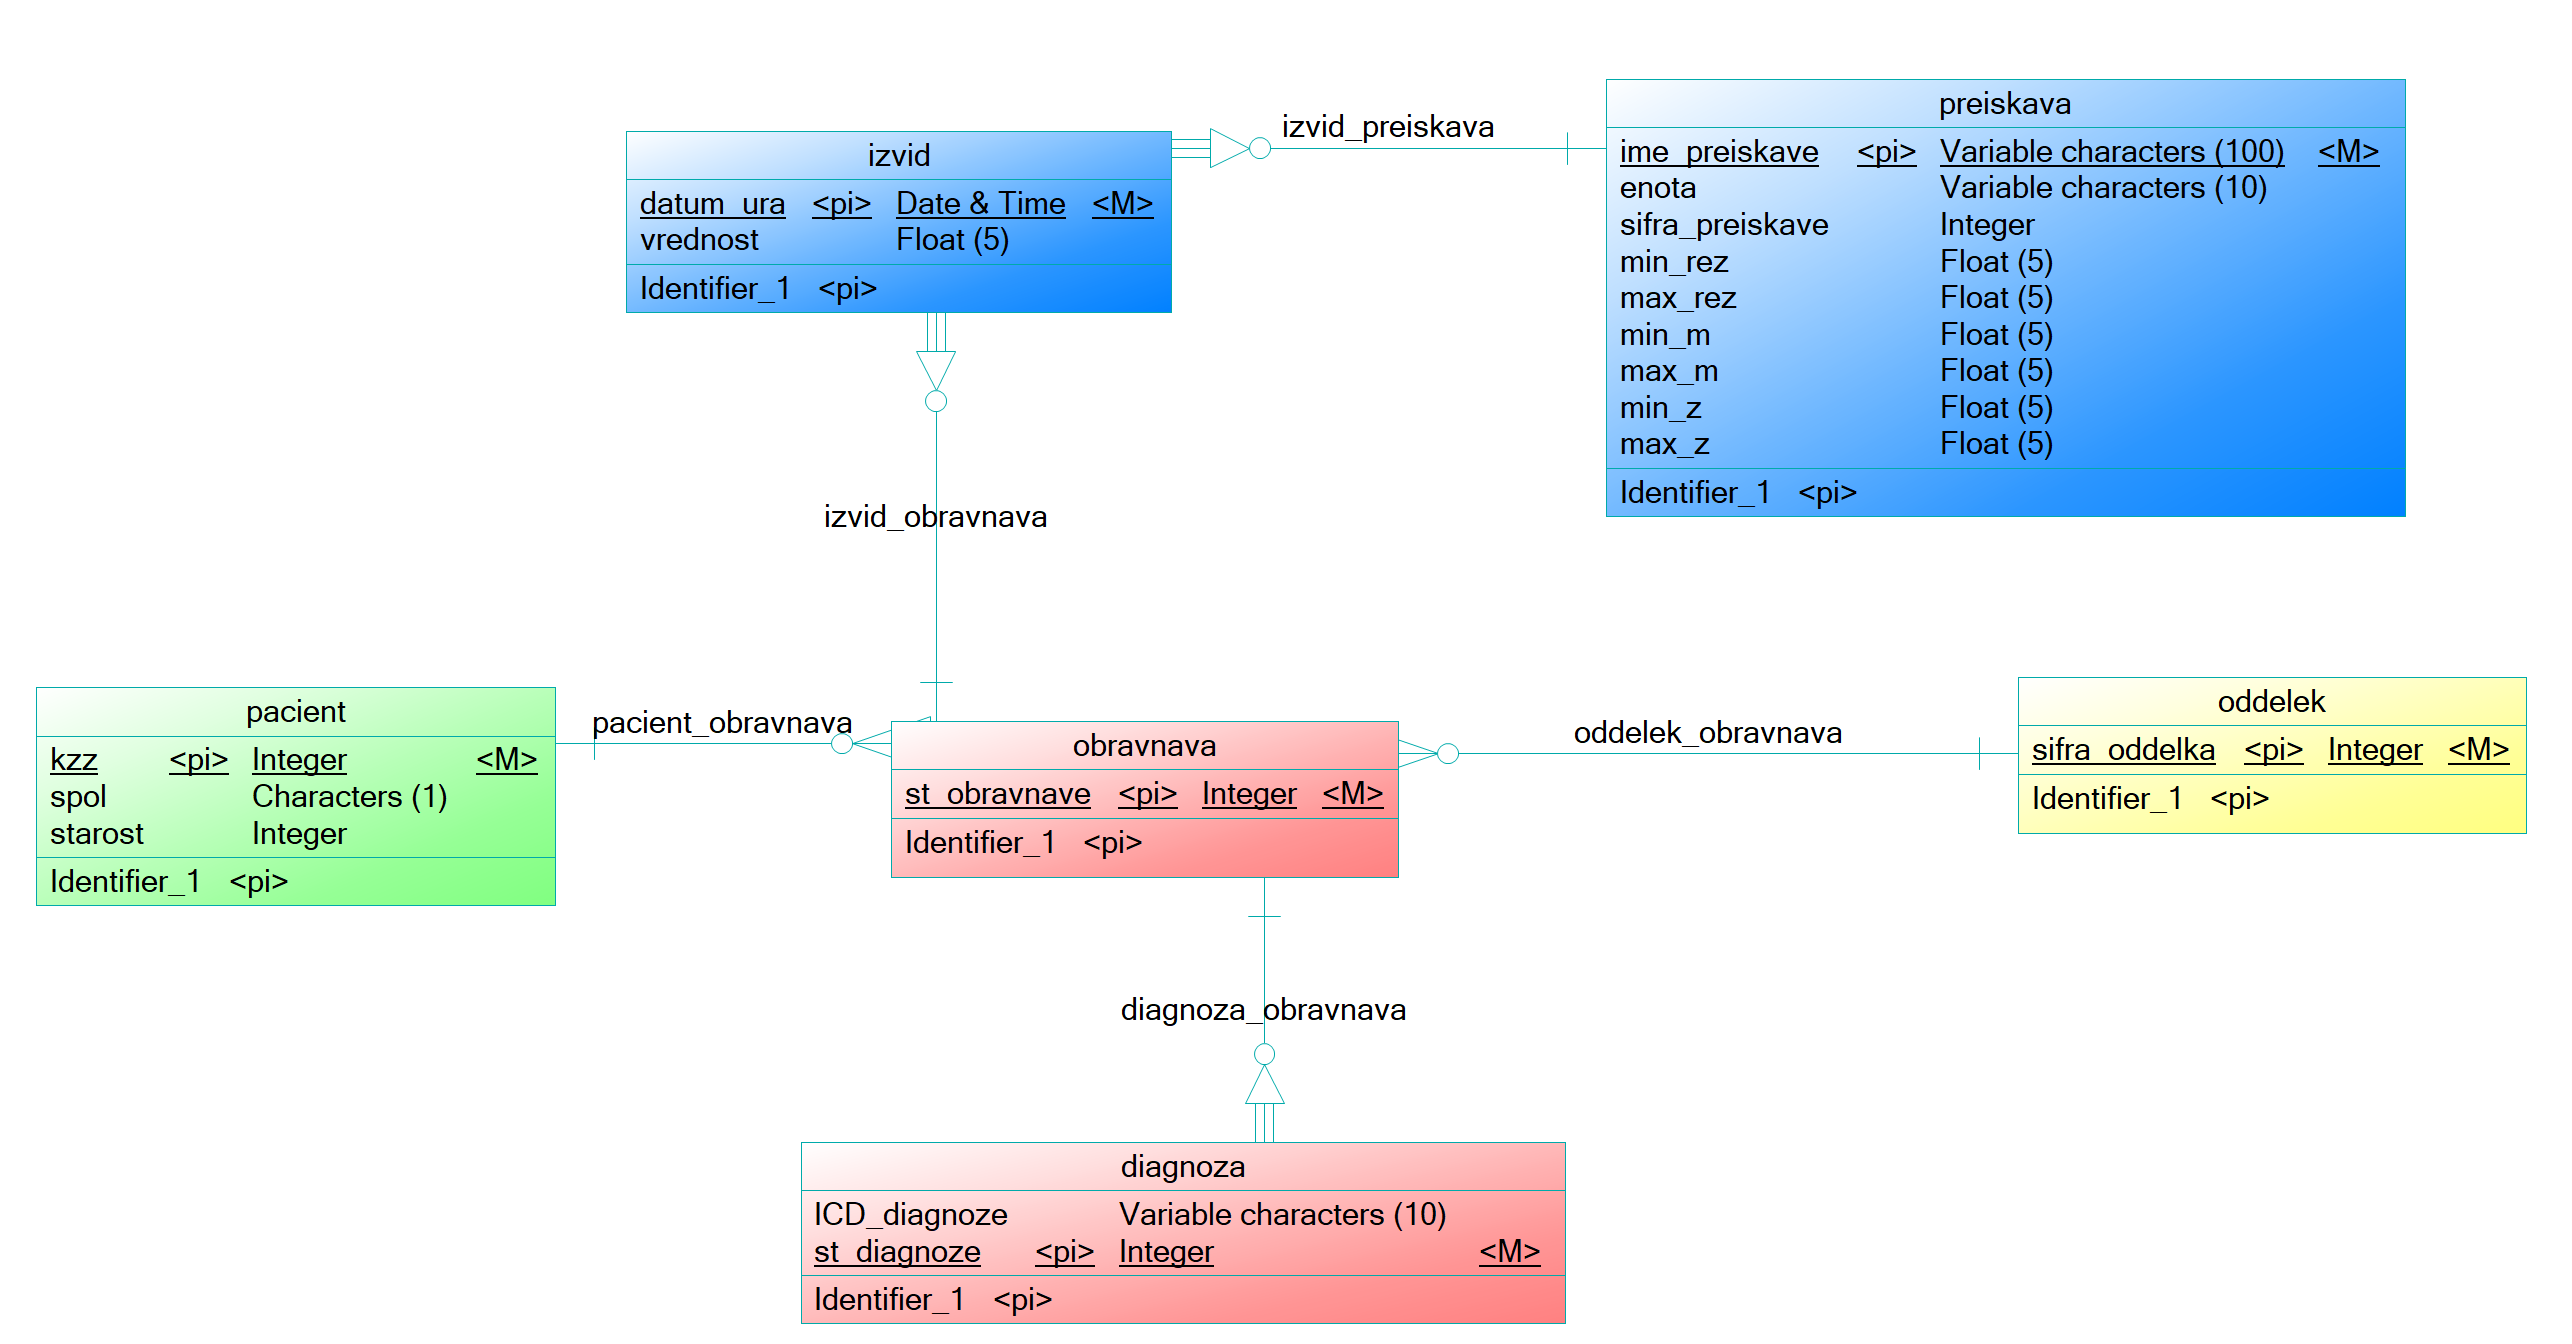
\includegraphics[width=\linewidth]{./pics/konceptni.png}
    \caption{Konceptni model podatkovne baze}
 \end{figure}

\subsection{Sestava podatkovne baze} 

\begin{center}
    \begin{tabular}{||l|r||}
        \hline
        \textbf{Tabela} & \textbf{Število zapisov v tabeli} \\
        \hline
        Pacient & 6 071 \\
        Obravnava & 6 643\\
        Diagnoza & 34 274\\
        Oddelek & 10\\
        Izvid & 846 906 \\
        Preiskava & 274\\
        \hline
    \end{tabular}
\end{center}

\section{Fizični model}
\subsection{MySQL}
\begin{figure}[htb]
   \noindent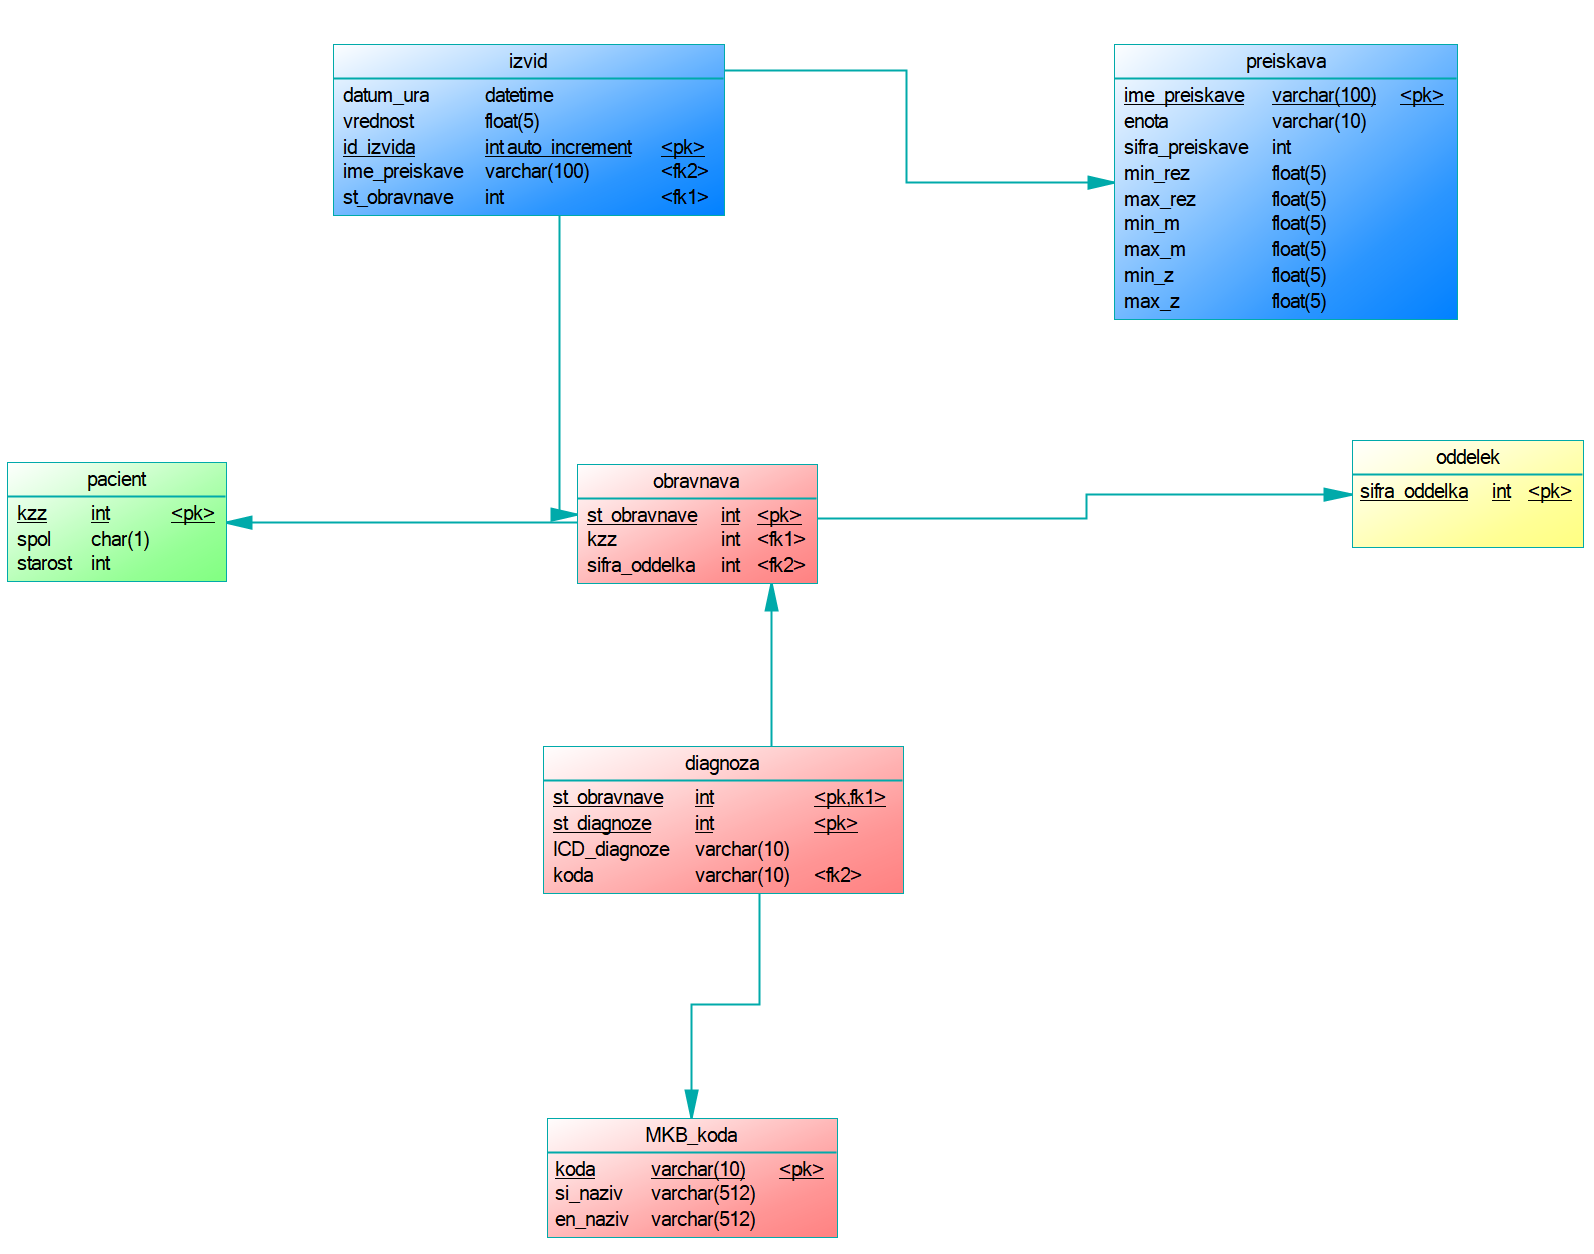
\includegraphics[width=\linewidth]{./pics/fizicni-mysql.png}
   \caption{Fizični model podatkovne baze za MySQL}
\end{figure}
Skripta za ustvarjanje podatkovne baze je shranjena v datoteki \textit{\underline{./sql-skripte/mysql-init.sql}}.

\subsection{PostgreSQL}
\begin{figure}[htb]
   \noindent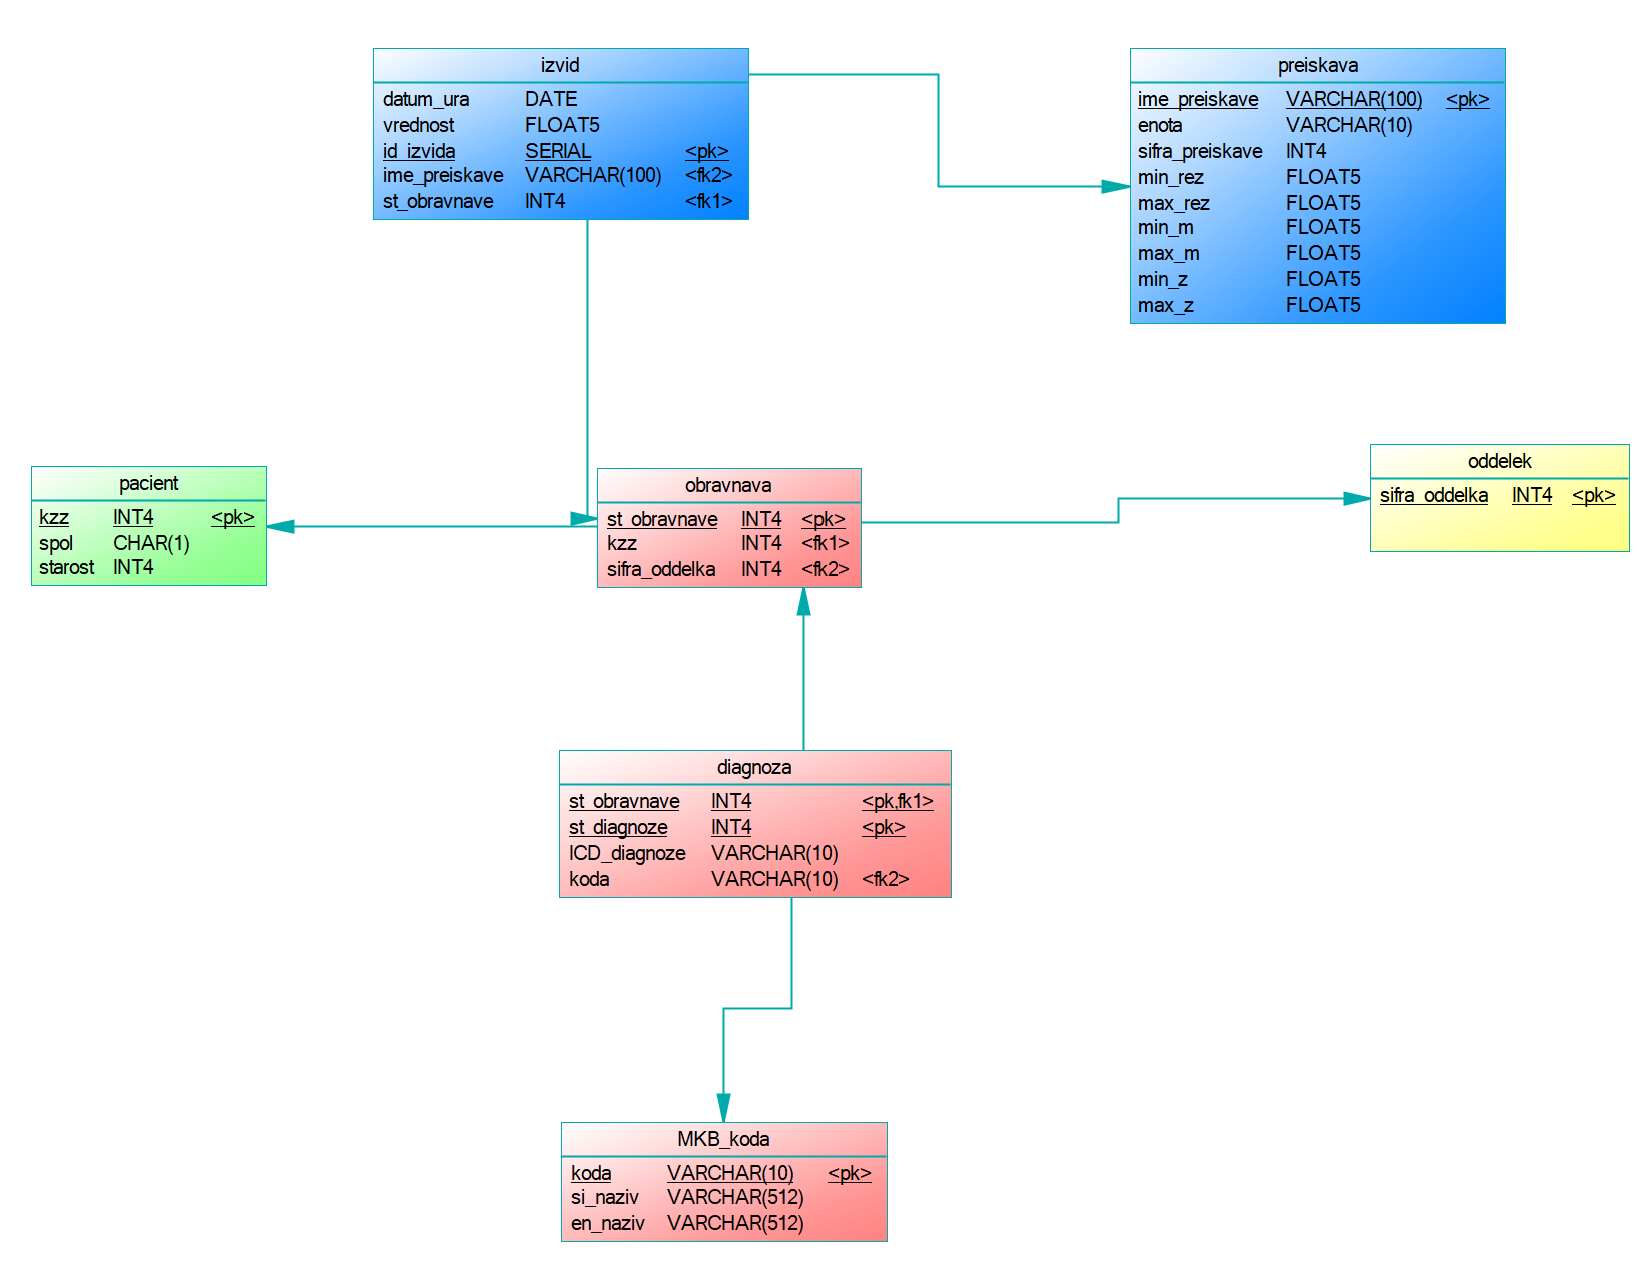
\includegraphics[width=\linewidth]{./pics/fizicni-postgres.png}
   \caption{Fizični model podatkovne baze za PostgreSQL}
\end{figure}
Skripta za ustvarjanje podatkovne baze je shranjena v datoteki \textit{\underline{./sql-skripte/postgres-init.sql}}.

\subsection{Microsoft SQL Server}
\begin{figure}[htb]
   \noindent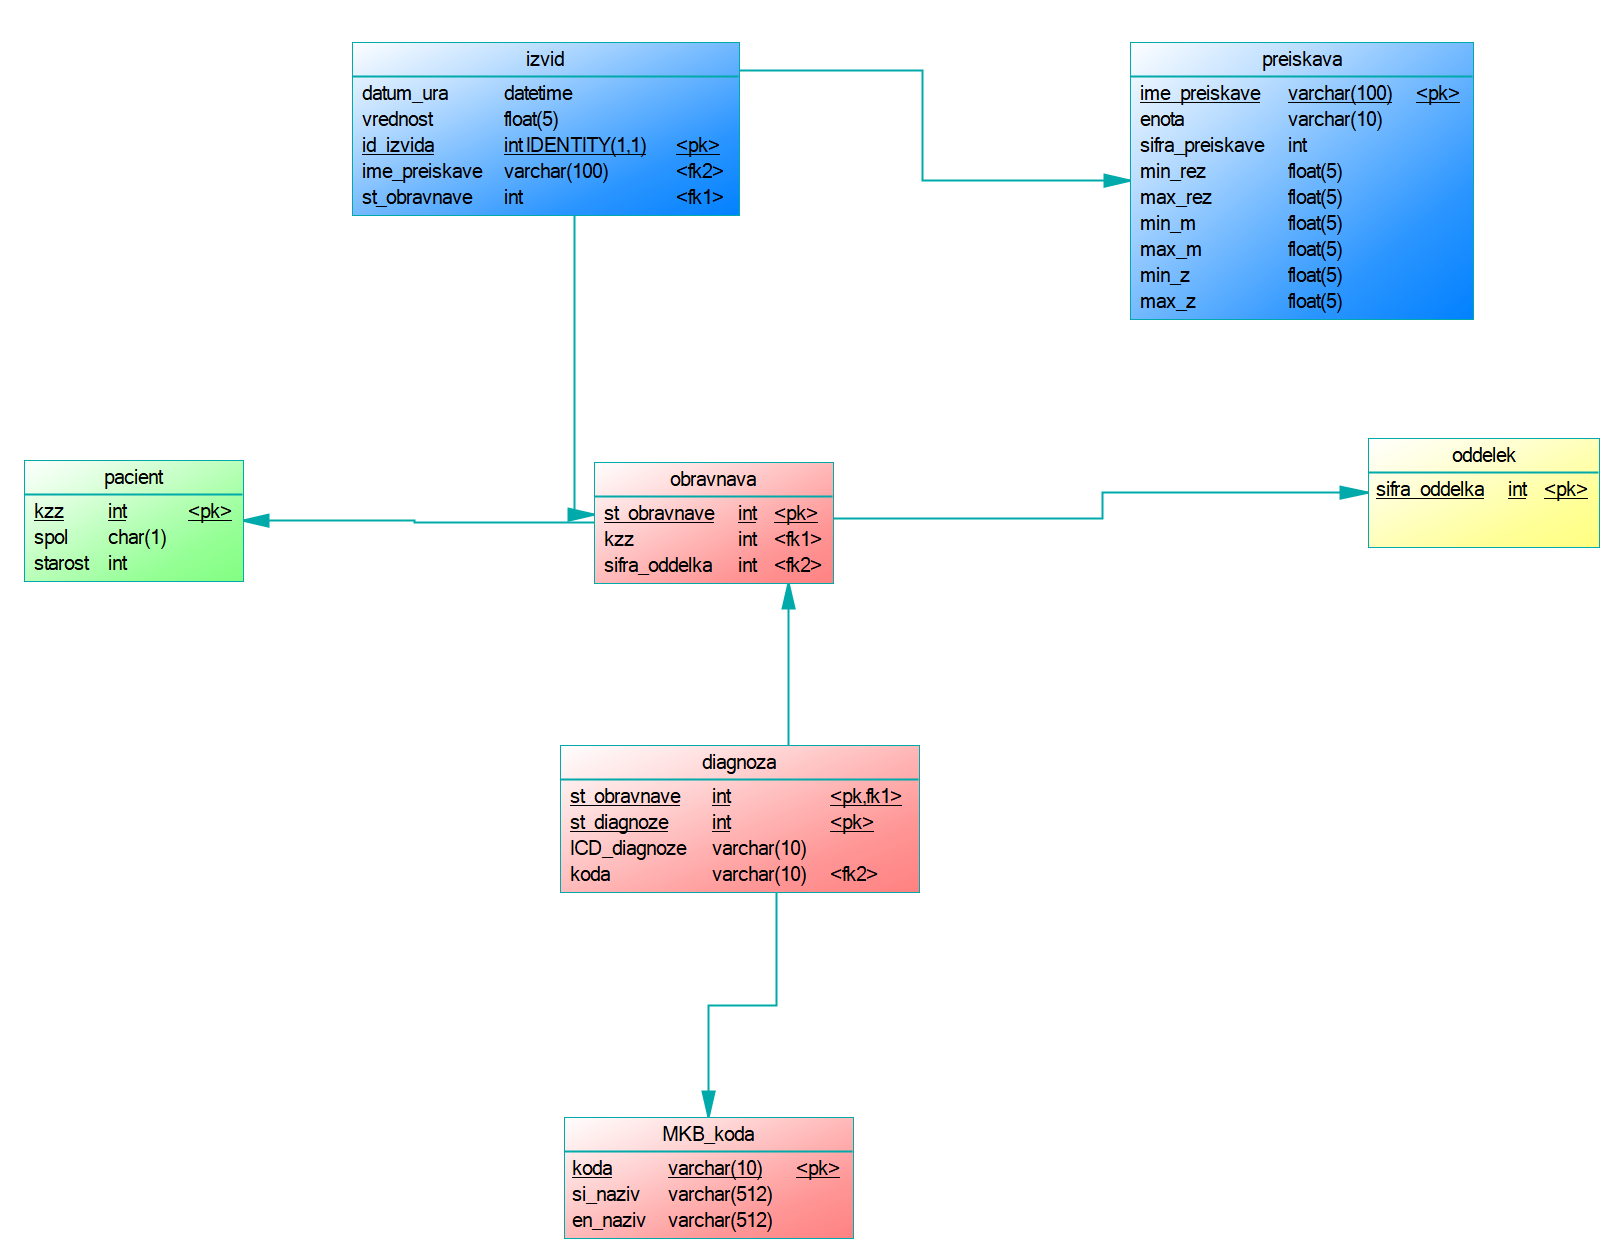
\includegraphics[width=\linewidth]{./pics/fizicni-mssql.png}
   \caption{Fizični model podatkovne baze za MS SQL Server}
\end{figure}
Skripta za ustvarjanje podatkovne baze je shranjena v datoteki \textit{\underline{./sql-skripte/mssql-init.sql}}.

\chapter{Testiranje}

\section{Kreiranje podatkovne baze}

\section{Vstavljanje (velike količine) zapisov v podatkovno bazo}

V podatkovno bazo se je vstavilo skupaj xxx zapisov. Vstavljanje je potekalo prek Python skripte filanje.py po postopku: 

\begin{enumerate}
   \item Iz csv (coma seperated values) datoteke je program prebral vrstico, jo razdeli in pretvoril v pravilen zapis spremelnjivke (s pomočjo vgrajenih ali pomožnih funkcij)
   \item Program shrani trenutni sistemski čas
   \item Program izvede INSERT
   \item Program od trenutnega sistemskega časa odšteje sistemski čas iz točke 3 in ga prišeje k števcu skupnega časa 
   \item Program se premakne na naslednjo vrstico csv datoteke
   \item Ko program obdela vse datoteke, funkcija vrne celoten seštevek časov izvajanja
\end{enumerate}
Test se je avomatsko izvedel desetkrat na vseh treh testnih bazah desetkrat v vrstnem redu: Microsoft SQL Server, MySql in PostgreSQL. Po vrsti je program polnil tabele:
\begin{enumerate}
   \item Pacient
   \item Oddelek
   \item Obravnava
   \item MKB\_koda
   \item Diagnoza
   \item Preiskava
   \item Izvid
\end{enumerate}

Po polnjenju vseh treh podatkovnih baz je program podatkovne baze izpraznil pri čemer je bil uporabljen ukaz \textit{DELETE * FROM |ime tabele| }. 
\\\\
Pri obdelavi rezultatov se najboljši in najslabši čas nista upoštevala, iz ostalih pa se je izračunalo povprečje.

\begin{center}
   \begin{tabular}{||c|c|c|c||}
      \hline
      \textbf{SUPB} & \textbf{Najboljši čas [s]} & \textbf{Najslabši čas [s]} & \textbf{Povprečje [s]} \\
      \hline
      \hline
      PostgreSQL & 512,716 & 520,791 & 515,921 \\
      Microsoft SQL Server & 592,745 & 608,040 & 596,453 \\
      MySQL & 619,255 & 630,775 & 623,806\\
      \hline
   \end{tabular}
\end{center}

\begin{figure}[htb]
   \noindent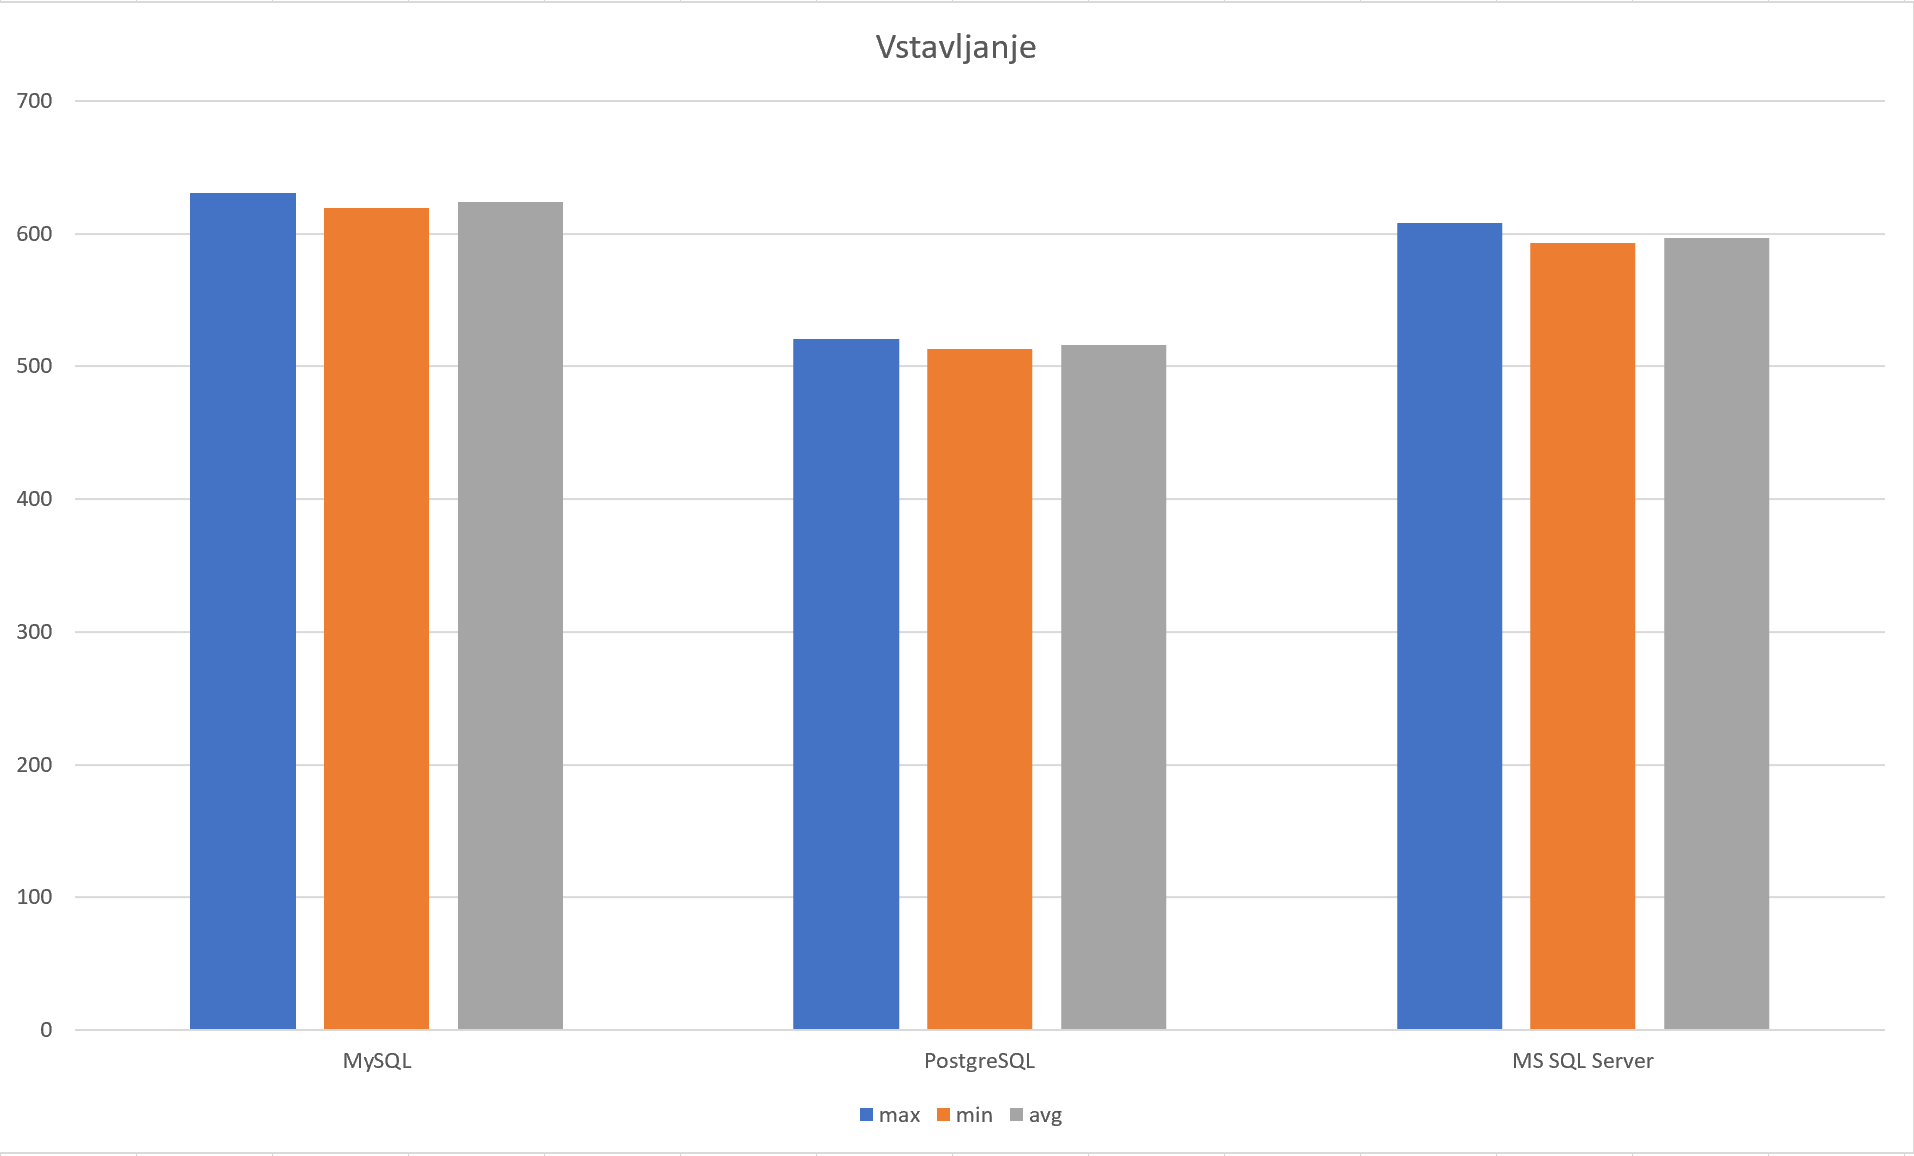
\includegraphics[width=\linewidth]{./pics/vstavljanje001.png}
   \caption{Primerjava "best, worst \& average" vstavljanja}
\end{figure}

\pagebreak

Iz rezultatov lahko vidimo, da je povprečje PostgreSQL-a ne le najboljše, ampak je celo za \textit{15 \%} 
boljši od najboljšega časa naslednjega zasledovalca, tj. Microsoft SQL Server, in za \textit{20\%} od MySQL.
\\\\
V povprečju je sicer PostgreSQL potreboval približno 8 minut in pol, Microsoft SQL Server nekaj manj, MySql pa nekaj več kot 10 minut.
\\\\
Ob tem gre poudariti, da se je pri vseh uporabljal \textit{običajen INSERT} in ne kakšna posebna oblika vstavljanja velike količine podatkov (npr. \textit{BULK INSERT} pri Microsoft SQL Server).
\\\\
Iz zgoraj navedenih rezultatov se, kot je zapisano v sekciji 1.4.1, določi točke po naslednjem ključu:

\begin{center}
   \begin{tabular}{||c|c|c|c||}
      \hline
      \textbf{SUPB} & Rezultat testiranja & Odstotek točk [\%] & Število točk\\
      \hline
      \hline
      PostgreSQL & 515,921 & 100 & 25\\
      Micorsoft SQL Server & 596,453 & 86,5 & 21,6\\
      MySql & 623,806 & 82,7 & 20,7\\
      \hline
   \end{tabular}
\end{center}

\section{Brisanje (velike količine) podatkov iz podatkovne baze}
Brisanje podatkov je potekalo avtomatsko z uporabo Python skripte \textit{filanje.py}. Testiranje se je izvedlo destkrat.
\\\\

Testiranje je potekalo po naslednjem postopku:
\begin{enumerate}
   \item Program za izvede ukaz s katerim pridobi imena vseh tabel v podatkovni bazi
   \item Program za vsako izmed tabel izvede:
      \item Program shrani trenutni sistemski čas
      \item Program izvede ukaz \textit{DELETE FROM |ime-tabele|}
      \item Program od trenutnega sistemskega časa odšteje shranjen čas
   \item Program vrne seštevek vsote časov izvajanja funkcije brisanja podatkov
\end{enumerate}

Rezultati izračunani iz povprečja so naslednji:
\begin{center}
   \begin{tabular}{||c|c|c|c||}
      \hline
      \textbf{SUPB} & \textbf{Testiranje [ms]} & \textbf{Odstotek točk [\%] } & \textbf{Število točk}\\
      \hline
      \hline
      Microsoft SQL Server & 1,087 & 100 & 25\\
      PostgreSQL & 1,490 & 72,9 & 18,2\\
      MySQL & 5,373 & 20,2 & 5,1\\
      \hline
   \end{tabular}
\end{center}

Iz zgornjih rezultatov lahko sklepamo, da je brisanje podatkov iz podatkovne baze veliko hitrejši postopek od vstavljanja.
Ravno zaradi tega so relativne razlike med testiranimi SUPB-ji izjemno velike v primerjavi z razlikami pri vstavljanju, čeprav
so absolutne razlike (predvsem med MS SQL Server in PostgreSQL) zanemarljive.

\section{Branje podatov iz podatkovne baze}
\subsection{Povezovanje tabel in primerjava med \textit{WHERE} in \textit{INNER JOIN}}

\paragraph{SQL poizvedba}
Poizvedba za vsakega izmed pacientov prikaže pacientovo številko zdravstvenega zavarovanja, spol, številko obravnave
ter kakšna vrsta preiskave je bila opravljena in njeno vrednost. V testiranju sta bili uporabljeni dve različni poizvedbi
ena z uporabo \textit{INNER JOIN} (poizvedba 1) in druga z uporabo \textit{WHERE} stavka (poizvedba 2).
\begin{lstlisting}[language = SQL]
Poizvedba 1:
   select
      p.kzz,
      p.spol,
      o.st_obravnave,
      i.ime_preiskave,
      i.vrednost
   from pacient p
   inner join obravnava o on o.kzz = p.kzz
   inner join izvid i on i.st_obravnave=o.st_obravnave
   order by p.kzz, o.st_obravnave
\end{lstlisting}

\begin{lstlisting}[language = SQL]
Poizvedba 2:
   select
       p.kzz,
       p.spol,
       o.st_obravnave,
       i.ime_preiskave,
       i.vrednost
   from
        pacient p,
        obravnava o,
        izvid i
   where
       p.kzz = o.kzz and
       o.st_obravnave = i.st_obravnave
   order by p.kzz, o.st_obravnave
\end{lstlisting}

\paragraph{Rezultati poizvedbe 1 (\textit{INNER JOIN})}
Test se je izvedel desetkrat, avtomatsko z uporabo Python skripte \textit{poizvedbe.py} za vse tri podatkovne baze.

\begin{center}
   \begin{tabular}{||c|c|c|c||}
      \hline
      \textbf{SUPB} & \textbf{Najboljši [ms]} & \textbf{Najslabši [ms]} & \textbf{Povprečen rezultat [ms]}\\
      \hline
      \hline
      Microsoft SQL Server & 361 & 389 & 372 \\
      MySql & 710 & 842 & 782 \\
      PostgreSQL & 1052 & 1352 & 1135\\
      \hline
   \end{tabular}
\end{center}
Primerjava hitrsoti izvedbe SQL stavka z uporabo \textit{INNER JOIN}

\paragraph{Rezultati poizvedbe 1 (\textit{WHERE})}
\begin{center}
   \begin{tabular}{||c|c|c|c||}
      \hline
      \textbf{SUPB} & \textbf{Najboljši [ms]} & \textbf{Najslabši [ms]} & \textbf{Povprečen rezultat [ms]}\\
      \hline
      \hline
      Microsoft SQL Server & 367 & 420 & 393 \\
      MySql & 795 & 1000 & 874 \\
      PostgreSQL & 1056 & 1313 & 1085\\
      \hline
   \end{tabular}
\end{center}
Primerjava hitrsoti izvedbe SQL stavka z uporabo \textit{WHERE}
\\\\
Microsoft SQL Server je tako pri poizvedbi 1 kot pri poizvedbi 2 za (vsaj) \(41\%\) hitrejši od MySql ter vsaj \(60\%\) od PostgreSQL, 
kateri se izkaže za veliko počasnejšega od konkurence.

Razlike med hitrostjo poizvedb pri uporabi \textit{WHERE} in \textit{INNER JOIN} so pri vseh treh bazah zanemarljive, vendar vseeno opazne.

\begin{center}
   \begin{tabular}{||c|c|c|c||}
      \hline
      \textbf{SUPB} & \textbf{\textit{INNER JOIN} [ms]} & \textbf{\textit{WHERE} [ms]} & \textbf{Razlika [\%]}\\
      \hline
      \hline
      Microsoft SQL Server & 392 & 372 & -4,5 \\
      MySql & 781 & 874 & 10,6 \\
      PostgreSQL & 1084 & 1135 & 7,7\\
      \hline
   \end{tabular}
\end{center}
Prikaz razlike v povprečni hitrosti izvedbe SQL poizvedbe z uporabo \textit{INNER JOIN} in \textit{WHERE} stavka.
\\\\
Relativne razlike v hitrosti so najmanj razvidne pri Microsoft SQL Server, kjer se zdi, da je \textit{WHERE} poizvedba bolje optimizirana, vendar so razlike premajhne, da bi lahko kaj takega trdili z dovolj veliko verjetnostjo.
Pri PostgreSQL in predvsem pri MySql se zdi, da je \textit{INNER JOIN} boljša izbira.

\paragraph{Določitev točk} Čeprav se poizvedba deli na dve sintaktično različni, je razultat obeh poizvedb identičen. Kot takega
ga torej štejemo kot eno postavko izračuna točk, pri čemer se upošteva boljši rezultat obeh poizvedb.

\begin{center}
   \begin{tabular}{||c|c|c|c||}
      \hline
      \textbf{SUPB} & \textbf{Testiranje} & \textbf{Odstotek točk [\%]} & \textbf{Število točk}\\
      \hline
      \hline
      Microsoft SQL Server & 372 & 100 & 50 \\
      MySql & 781 & 50,3 & 23,1 \\
      PostgreSQL & 1085 & 36,2 & 17,2\\
      \hline
   \end{tabular}
\end{center}

\subsection{Uporaba funkcije \textit{COUNT} v povezanih tabelah}
Test se je izvedel desetkrat, avtomatsko z uporabo Python skripte \textit{poizvedbe.py} za vse tri podatkovne baze.

\paragraph{SQL poizvedba}
Poizvedba izpiše ime preiskave in število izvidov, katerih vrednost je višja od priporočene vrednosti glede na spol.
Izpis je urejen padajoče po številu prekoračenih izvidov.
\begin{lstlisting}[language = SQL]
select
   i.ime_preiskave,
   count(i.ime_preiskave)
from
   izvid i
inner join obravnava o on 
      i.st_obravnave = o.st_obravnave
inner join pacient p 
      on p.kzz = o.kzz
inner join preiskava p2 
      on i.ime_preiskave = p2.ime_preiskave
where
   (p.spol = 'M' and p2.max_m <= i.vrednost 
      and p2.max_m is not null) 
   or
   (p.spol = 'Z' and p2.max_z <= i.vrednost 
      and p2.max_z is not null)
group by i.ime_preiskave
order by count(i.ime_preiskave) desc
\end{lstlisting}

\begin{center}
   \begin{tabular}{||c|c|c|c||}
      \hline
      \textbf{SUPB} & \textbf{Najboljši [ms]} & \textbf{Najslabši [ms]} & \textbf{Povprečen rezultat [ms]}\\
      \hline
      \hline
      PostgreSQL & 378 & 504 & 413 \\
      Microsoft SQL Server & 606 & 646 & 633 \\
      MySql & 1653 & 1778 & 1704\\
      \hline
   \end{tabular}
\end{center}

\begin{center}
   \begin{tabular}{||c|c|c|c||}
      \hline
      \textbf{SUPB} & \textbf{Testiranje} & \textbf{Odstotek točk [\%]} & \textbf{Število točk}\\
      \hline
      \hline
      PostgreSQL & 413 & 100 & 50\\
      Microsoft SQL Server & 633 & 65,2 & 32,6 \\
      MySql & 1704 & 24,2 & 12,1 \\
      \hline
   \end{tabular}
\end{center}


\end{document}